\subsection{Innovative task: Shortest Path}
{\bf Proof of Correctness: } In order to prove the correctness, we conduct experiments on a small dataset that we manually constucted. And the result is exactly the same. 

In order to test the performance of the SQL implementation, we run the shortest path algorithm on incrementally larger datasets, the
running time erquired according the size of graph is ploted in Figure \ref{sp:plot}. We can observe from that figure that as the graph size increases, the running time grows much faster than linear. The reason for this is that we implemented all the data structures through
tables, which incurs a lot of overhead of search. An alternative is to use the data types provided by Postgres. 

\begin{figure}[!htbf]
\begin{center}
\begin{tabular}{c}
     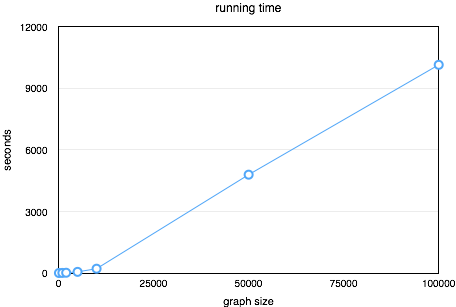
\includegraphics[width=0.7\textwidth]{FIG/sp_plot.png}
\end{tabular}
\caption{Running time VS graph size}
\label{sp:plot}
\end{center}
\end{figure}